% !BIB TS-program = biber

\RequirePackage[l2tabu,orthodox]{nag}

% TODO: decide if one-sided/two-sided
%\documentclass[headsepline,footsepline,footinclude=false,fontsize=11pt,paper=a4,listof=totoc,bibliography=totoc,BCOR=12mm,DIV=12]{scrbook} % two-sided
\documentclass[headsepline,footsepline,footinclude=false,oneside,fontsize=11pt,paper=a4,listof=totoc,bibliography=totoc]{scrbook} % one-sided

% TODO: change thesis information
\newcommand*{\getUniversity}{Universidad Autónoma de Madrid}
\newcommand*{\getFaculty}{Escuela Politécnica Superior}
\newcommand*{\getDegree}{Data Science}
\newcommand*{\getSchool}{Escuela Politécnica Superior}
\newcommand*{\getTitle}{Automated Exploration and Profiling of Conversational Agents}
\newcommand*{\getTitleGer}{Titel der Abschlussarbeit}
\newcommand*{\getAuthor}{Iván Sotillo del Horno}
\newcommand*{\getDoctype}{Master's}
\newcommand*{\getSupervisor}{Juan de Lara Jaramillo}
\newcommand*{\getCoSupervisor}{Esther Guerra Sánchez}
\newcommand*{\getDepartment}{Department of Computer Science}
\newcommand*{\getLogo}{logos/logo_uameps_color.png}
\newcommand*{\getAdvisor}{Advisor}
\newcommand*{\getKeywords}{keyword;another keyword;one more}
\newcommand*{\getSubmissionDate}{\today}
\newcommand*{\getSubmissionLocation}{Madrid, Spain}

% TODO: change citation style in settings
\PassOptionsToPackage{table,svgnames,dvipsnames}{xcolor}

\usepackage{fontspec}           % Main package for using system fonts with Lua/XeTeX
\usepackage[english]{babel}      % Language support for hyphenation rules, etc.
\usepackage{csquotes}             % Context-sensitive quotation marks


\setmainfont{TeX Gyre Pagella}
\setsansfont{TeX Gyre Heros}
\setmonofont{TeX Gyre Cursor}

\usepackage{unicode-math}
\setmathfont{TeX Gyre Pagella Math}

\usepackage[%
  backend=biber,
  style=ieee,
  citestyle=numeric-comp,
  bibstyle=ieee,
  sorting=none,
  maxnames=3,
  minnames=1,
  maxbibnames=99,
  giveninits=true,
  uniquename=init]{biblatex} % IEEE style for citations
\usepackage{graphicx}
\usepackage{scrhack} % necessary for listings package
\usepackage{listings}
\usepackage{lstautogobble}
\usepackage{tikz}
\usepackage{pgfplots}
\usepackage{pgfplotstable}
\usepackage{booktabs}
\usepackage[final]{microtype}
\usepackage{caption}
\usepackage[printonlyused]{acronym}
\usepackage{ifthen}
\usepackage{hyperref} % Added for autoref support
\usepackage{tcolorbox}
\usepackage{tabularx}
\usepackage{makecell}
\usepackage{ragged2e}


%\hypersetup{hidelinks} % removes colored boxes around references and links

% for fachschaft_print.pdf
\makeatletter
\if@twoside
	\typeout{TUM-Dev LaTeX-Thesis-Template: twoside}
\else
	\typeout{TUM-Dev LaTeX-Thesis-Template: oneside}
\fi
\makeatother

\addto\extrasenglish{
	\def\lstnumberautorefname{Line}
	\def\chapterautorefname{Chapter}
	\def\sectionautorefname{Section}
	\def\subsectionautorefname{Subsection}
	\def\subsubsectionautorefname{Subsubsection}
}

% Themes
\ifthenelse{\equal{\detokenize{dark}}{\jobname}}{%
  % Dark theme
  \newcommand{\bg}{black} % background
  \newcommand{\fg}{white} % foreground
  \usepackage[pagecolor=\bg]{pagecolor}
  \color{\fg}
}{%
  % Light theme
  \newcommand{\bg}{white} % background
  \newcommand{\fg}{black} % foreground
}

%\bibliography{bibliography}
\addbibresource{bibliography.bib}

\setkomafont{disposition}{\normalfont\bfseries} % use serif font for headings
\linespread{1.05} % adjust line spread for mathpazo font

% Add table of contents to PDF bookmarks
%\BeforeTOCHead[toc]{{\cleardoublepage\pdfbookmark[0]{\contentsname}{toc}}}

% Define TUM corporate design colors
% Taken from http://portal.mytum.de/corporatedesign/index_print/vorlagen/index_farben
\definecolor{TUMBlue}{HTML}{0065BD}
\definecolor{TUMSecondaryBlue}{HTML}{005293}
\definecolor{TUMSecondaryBlue2}{HTML}{003359}
\definecolor{TUMBlack}{HTML}{000000}
\definecolor{TUMWhite}{HTML}{FFFFFF}
\definecolor{TUMDarkGray}{HTML}{333333}
\definecolor{TUMGray}{HTML}{808080}
\definecolor{TUMLightGray}{HTML}{CCCCC6}
\definecolor{TUMAccentGray}{HTML}{DAD7CB}
\definecolor{TUMAccentOrange}{HTML}{E37222}
\definecolor{TUMAccentGreen}{HTML}{A2AD00}
\definecolor{TUMAccentLightBlue}{HTML}{98C6EA}
\definecolor{TUMAccentBlue}{HTML}{64A0C8}
\definecolor{EPS}{HTML}{996114}
\definecolor{UAMGreen}{HTML}{4a7729}
\definecolor{UAMBlue}{HTML}{0077c8}

% Settings for pgfplots
\pgfplotsset{compat=newest}
\pgfplotsset{
  % For available color names, see http://www.latextemplates.com/svgnames-colors
  cycle list={TUMBlue\\TUMAccentOrange\\TUMAccentGreen\\TUMSecondaryBlue2\\TUMDarkGray\\},
}

% Settings for lstlistings
\lstset{%
  basicstyle=\ttfamily,
  columns=fullflexible,
  autogobble,
  keywordstyle=\bfseries\color{TUMBlue},
  stringstyle=\color{TUMAccentGreen},
  captionpos=b
}

\usepackage[absolute,overlay]{textpos}
\setlength{\TPHorizModule}{1cm}
\setlength{\TPVertModule}{1cm}

\begin{document}

% Set page numbering to avoid "destination with the same identifier has been already used" warning for cover page.
% (see https://en.wikibooks.org/wiki/LaTeX/Hyperlinks#Problems_with_Links_and_Pages).
\pagenumbering{alph}
%\begin{titlepage}
  % HACK for two-sided documents: ignore binding correction for cover page.
  % Adapted from Markus Kohm's KOMA-Script titlepage=firstiscover handling.
  % See http://mirrors.ctan.org/macros/latex/contrib/koma-script/scrkernel-title.dtx,
  % \maketitle macro.
  \oddsidemargin=\evensidemargin\relax
  \textwidth=\dimexpr\paperwidth-2\evensidemargin-2in\relax
  \hsize=\textwidth\relax

  % --- 1. Logo ---
  \begin{flushleft}
    \includegraphics[width=90mm]{\getLogo}
  \end{flushleft}

  \vfill % Replaced fixed vspace with vfill for better vertical distribution

  % --- 2. Document Type ---
  \begin{center}
    {\Large\bfseries\MakeUppercase{MASTER'S THESIS}} \par
  \end{center}

  \vspace{2cm}

  % --- 3. Thesis Title ---
  \begin{center}
    \begin{minipage}{0.8\textwidth}
      \centering
      {\huge\bfseries \getTitle{} \par}
    \end{minipage}
  \end{center}

  \vspace{2cm}

  % --- 4. Master's Program ---
  \begin{center}
    {\Large\bfseries Master's in \getDegree{}}
  \end{center}

  \vfill % Replaced fixed vspace with vfill to push content apart

  % --- 5. Author, Supervisor, and Date Block ---
  \begin{center}
    \begin{tabular}{r @{\hspace{1.5cm}} l}
      \bfseries Author: & \large\getAuthor{} \\[12pt]
      \bfseries Supervisor: & \large\getSupervisor{} \\[12pt]
      \bfseries Co-supervisor: & \large\getCoSupervisor{} \\[12pt]
      \bfseries Department: & \large\getDepartment{} \\[24pt] % Extra space before date
      \bfseries DATE: & \large\getSubmissionDate{} \\
    \end{tabular}
  \end{center}

  \vfill

  % --- 6. Footer ---
  \begin{textblock}{15}(1,28.2) % exact values for positioning the footer
    \noindent
    \textcolor{UAMBlue}{
      \small \getUniversity{} \\
      \small \getFaculty{}
    }
  \end{textblock}

\end{titlepage}
 basically we have it at the title page

\frontmatter{}

\begin{titlepage}
  \centering

  % Logo with better spacing
  \includegraphics[width=100mm]{\getLogo}
  \vspace{15mm}

  % Document type with improved styling
  \begin{center}
    {\Large\bfseries\MakeUppercase{\getDoctype{}}} \par
    \vspace{2mm}
    {\color{gray}\rule{0.3\textwidth}{0.5pt}} % Decorative line
  \end{center}

  \vspace{12mm}

  % Title with enhanced typography
  {\huge\bfseries \getTitle{} \par}

  \vspace{15mm}

  % Subtitle with better spacing
  {\Large\itshape \getDoctype{} in \getDegree{} \par}

  \vspace{20mm}

  % Information table with improved formatting
  \begin{tabular}{@{}r @{\hspace{8mm}} l@{}}
    \textbf{Author:}          & \getAuthor{}         \\[2mm]
    \textbf{Supervisor:}      & \getSupervisor{}     \\[2mm]
    \textbf{Co-supervisor:}   & \getCoSupervisor{}   \\[2mm]
    \textbf{Department:}      & \getDepartment{}     \\[2mm]
    \textbf{Submission Date:} & \getSubmissionDate{} \\
  \end{tabular}

  \vfill

  % University information with enhanced styling
  \textcolor{UAMBlue}{
    \begin{center}
      {\large\bfseries \getUniversity{}} \\[1mm]
      {\normalsize \getFaculty{}}
    \end{center}
  }

\end{titlepage}

\thispagestyle{empty}
\vspace*{0.8\textheight}
\noindent
I confirm that this \MakeLowercase{\getDoctype{}} is my own work and I have documented all sources and material used.

\vspace{15mm}
\noindent
\getSubmissionLocation{}, \getSubmissionDate{} \hspace{\fill} \getAuthor{}

\cleardoublepage{}

\addcontentsline{toc}{chapter}{Acknowledgments}
\thispagestyle{empty}

\vspace*{20mm}

\begin{center}
{\usekomafont{section} Acknowledgments}
\end{center}

\vspace{10mm}

%TODO: Acknowledgments

\cleardoublepage{}

\chapter{\abstractname}

Conversational agents, or chatbots,
have become a key component of modern software ecosystems,
yet their complex, non-deterministic, and heterogeneous nature
presents significant challenges for quality assurance.
Existing testing methodologies
often require source code access,
depend on manually created test scripts or pre-existing conversational corpora,
or are tied to specific development frameworks.
These limitations create a significant bottleneck
for the automated, black-box testing of deployed systems.

This thesis presents \acf{TRACER},
a methodology and open-source framework
for the automated exploration, modelling, and profiling of conversational agents.
\ac{TRACER} employs a \ac{LLM}-powered agent
to systematically interact with a deployed chatbot in a black-box manner,
automatically inferring a structured functional model of its capabilities.
This model captures the chatbot's
conversational workflows, supported parameters, and expected outputs.
From this inferred model,
\ac{TRACER} then automatically synthesises
a comprehensive set of detailed test user profiles,
designed for execution by a user simulator.
The entire methodology is supported by a full-stack web application
that provides easy access to the end-to-end workflow
from model inference with \ac{TRACER} to test execution with the SENSEI user simulator.

We validate the effectiveness of the approach through three research questions.
In a controlled, white-box environment using four open-source chatbots,
the first experiment demonstrated that \ac{TRACER} achieves high functional coverage.
In the second experiment,
the synthesised profiles successfully detected 84.6\% of injected faults in a mutation testing analysis.
In a black-box evaluation against five real-world, deployed chatbots,
the models inferred by \ac{TRACER} achieved an average precision of 96.0\% upon manual verification.
The results demonstrate that \ac{TRACER} provides a robust, practical, and effective solution
that significantly advances the state of the art in automated, black-box testing for modern conversational agents.

\microtypesetup{protrusion=false}
\tableofcontents{}
\microtypesetup{protrusion=true}

\mainmatter{}

% !TeX root = ../main.tex
% Add the above to each chapter to make compiling the PDF easier in some editors.

\chapter{Introduction}\label{chapter:introduction}

\section{Context}

The growth of conversational agents, popularly known as chatbots,
has changed the way humans interact with computers across a range of domains.
From general-purpose assistants like OpenAI's ChatGPT \autocite{ChatGPT} or Google's Gemini \autocite{GoogleGemini} to task-oriented agents that assist users in particular tasks such as shopping or customer service.
Such systems provide natural language interaction with services from customer service and e-commerce websites to educational materials.
The spread of these agents has also been accelerated by developments in generative \ac{AI}, particularly \acp{LLM} \autocite{minaeeLargeLanguageModels2025}, which have dramatically improved chatbot functionality, enabling them to both generate and comprehend natural language without explicitly programmed rules.

\section{Motivation}

The increasing prevalence of these systems has heightened concerns about their correctness, reliability, and quality assurance.
As these systems become ubiquitous in areas like healthcare or finance, which demand high levels of trust, the requirement for validation and testing becomes paramount.
Nevertheless, the heterogeneity of chatbot building approaches,
with intent-based platforms such as Google's Dialogflow \autocite{Dialogflow} or Rasa \autocite{Rasa2020}, multi-agent programming environments based on \acp{LLM} like LangGraph \autocite{LangGraph} and Microsoft's AutoGen \autocite{AutoGen}, and \acp{DSL} such as Taskyto \autocite{sanchezcuadradoAutomatingDevelopmentTaskoriented2024},
presents significant challenges in seeking an overarching methodology to test these systems.


Conventional software testing methods \autocite{ammannIntroductionSoftwareTesting2017}
are hardly applicable to chatbot systems.
The intricacy of \ac{NLP}, the non-deterministic nature of \acp{LLM} and the dynamic flow of a real conversation make traditional testing insufficient for dialogue agents.
Although there have been some methods for developing testing methods for chatbots \cite{cuadradoIntegratingStaticQuality2024, canizaresMeasuringClusteringHeterogeneous2024}, they often focus on particular chatbot technologies \autocite{RasaTest2025}, require substantial manual effort including the provision of test conversations \autocite{CyaraBotium, RasaTest2025} or synchronous human interaction \autocite{renEvaluationTechniquesChatbot2019}, rely on available conversation corpus \autocite{vasconcelosBottesterTestingConversational2017}, or require access to the source code of the chatbot \autocite{canizaresCoveragebasedStrategiesAutomated2024, gomez-abajoMutationTestingTaskOriented2024, urricoMutaBotMutationTesting2024}, thus restricting their applicability to deployed systems as black boxes.

\section{Objectives}

The work in this thesis seeks to address these issues by the development of Task Recognition And Chatbot ExploreR (\ac{TRACER}), a tool for extracting comprehensive models from deployed conversational agents, and then, with this model, generate user profiles that are test cases for a user simulator named SENSEI \autocite{delaraAutomatedEndtoEndTesting2025, delaraSensei}.
\ac{TRACER} uses an \ac{LLM} agent to systematically investigate the chatbot's abilities through natural language interactions, without requiring manual test case writing or access to the source code of the chatbot.
This black-box strategy facilitates automated generation of comprehensive chatbot models that capture supported languages, fallback mechanisms, functional capabilities, input parameters, acceptable parameter values, output data structures, and conversational flow patterns.


The extracted chatbot model serves as the foundation for the automated synthesis of test cases.
In particular, \ac{TRACER} produces user profiles that model varied users that interact with the chatbot through SENSEI \autocite{delaraAutomatedEndtoEndTesting2025, delaraSensei}, yet alternate implementations of \ac{TRACER} could be used to produce various kinds of test cases from the extracted model.
The combination of \ac{TRACER} and SENSEI results in a test approach that requires only a connector for the chatbot’s API.

In order to make this research accessible and reproducible, \ac{TRACER} has been developed as a full, open-source tool.
It is available publicly as a \ac{PyPI} package \autocite{sotillodelhornoChatbottracerToolModel} and can be installed using \texttt{pip install chatbot-tracer}.
The complete source code is available on GitHub \url{https://github.com/Chatbot-TRACER/TRACER}, and a dedicated web application has been created to offer an easy experience for the whole test pipeline, ranging from model extraction and user profiles generation with \ac{TRACER} to test execution with SENSEI.


To direct this inquiry, we have established the following research questions:
\begin{itemize}
\item \textbf{RQ1: How effective is TRACER in modelling chatbot functionality?}
  This question evaluates the capability of the proposed model discovery method to attain high functional coverage in a controlled environment where the ground truth is available.
\item \textbf{RQ2: How effective are the synthesised profiles at detecting faults in controlled environments?}
  This question tests the accuracy of the proposed method by applying mutation testing \autocite{gomez-abajoMutationTestingTaskOriented2024} to estimate the capacity of the created profiles to detect specific, injected faults.
\item \textbf{RQ3: How accurately does TRACER model the functionalities of real-world, deployed chatbots?}
  This question addresses the practical, real-world applicability of \ac{TRACER}.
  To answer it, we run \ac{TRACER} against a set of deployed chatbots,
  and then perform a manual verification of every functionality inferred.
  This allows us to measure the precision of the model,
  that is, the percentage of discovered functionalities that are correct and valid.
\end{itemize}

\section{Contributions}

The primary contribution of this thesis is the design, implementation and evaluation of \acf{TRACER},
a framework for the automated black-box testing of conversational agents.
\ac{TRACER} addresses the limitations by introducing a two-stage process:
it first automatically infers a model of a deployed chatbot through natural language interaction,
and then synthesises this model into a set of user profiles
that will executed with SENSEI \autocite{delaraSensei} to complete the evaluation of the chatbot.
All of this is supported by a web application that will enable users to easily execute TRACER and SENSEI intuitively.

The proposed \ac{TRACER}'s methodology and its experimental results presented in this thesis
have been peer-reviewed and accepted for a publication at the
37th International Conference on Testing Software and Systems (ICTSS)
\autocite{sotillodelhornoAutomatedExplorationConversational2025}.

This research has been partially funded by the SATORI project, supported by the Spanish Ministry of Science and Innovation.

\section{Thesis Organization}

The remainder of the thesis is organized as follows:
\autoref{chapter:state_of_the_art} sets up the context and state of the art of chatbot testing.
\autoref{chapter:tracer} lays out the primary methodology of how \ac{TRACER} extracts models from chatbots.
\autoref{chapter:user-profiles} explains the user profile structure, and the way \ac{TRACER} creates them.
\autoref{chapter:tool_support} illustrates \ac{TRACER} Command Line Interface (CLI) and web application for utilising both SENSEI and \ac{TRACER}.
\autoref{chapter:evaluation}
evaluates \ac{TRACER} to answer the research questions.
\autoref{chapter:conclusion}
summarizes the thesis and proposes lines for future work.

% !TeX root = ../main.tex
% Add the above to each chapter to make compiling the PDF easier in some editors.

\chapter{Background and State of the Art}\label{chapter:state_of_the_art}

%TODO: Hacer una intruducción al capítulo

\section{Background}

\subsection{Conversational Agents}

Conversational agents, commonly referred to as chatbots,
are software systems designed to interact with users through natural language dialogue.
These systems have evolved from simple rule-based programs that followed predefined conversation flows
to sophisticated AI-powered agents capable of understanding context, maintaining conversational state, and generating human-like responses.

Modern conversational agents can be categorized into two main types
given the domain and range of their capabilities.
\begin{itemize}
  \item \textbf{Task-oriented:} on one hand we have the task-oriented chatbots,
  these are designed to assist users in completing specific tasks, such as booking appointments, processing orders, or providing customer support.
  These systems typically follow structured conversation flows
and maintain explicit state management to track task progress.
  Examples of these chatbots are Taskyto \autocite{sanchezcuadradoAutomatingDevelopmentTaskoriented2024} or UAM's assistant Ada \autocite{AdaUAM}.

  \item \textbf{Open-domain:}
  on the other hand, open-domain chatbots
  engage in general conversation without specific task constraints,
  aiming to provide informative, helpful, or entertaining interactions across a wide range of topics.
  These are chatbots like ChatGPT \autocite{ChatGPT} or Gemini \autocite{GoogleGemini}.
\end{itemize}

The development of these conversational agents
has beeen facilitated by various frameworks and platforms.
\begin{itemize}
  \item \textbf{Intent-based frameworks:}
    these frameworks such as Google's Dialogflow \autocite{Dialogflow} or Rasa \autocite{Rasa2020}
    enable developers to define conversation flow through intents, utterances, and responses.
    These platforms have low latency and deterministic behavior
    but are very rigid, struggle to scale,
    and to work properly require a big corpus to be trained on.

  \item \textbf{Multi-agent programming environments:}
    these systems like LangGraph \autocite{LangGraph} or Microsoft's AutoGen \autocite{AutoGen},
    allow for the creating of complex conversational systems
    where multiple \ac{AI} agents collaborate to process the user's request.
    These frameworks make use of the capabilities of \acp{LLM}.
    While they are less rigid than the previous ones,
    they can suffer from hallucinations, 
    higher latency, and since they are not deterministic,
    getting out of the scope, and thus, making it harder to test it.
\end{itemize}

\subsection{\aclp{LLM}}

\aclp{LLM} represent a significant advancement in \acl{NLP},
enable conversational agents to understand and generate human-like text
without explit programming of conversational rules like in intent-based frameworks.
These models, trained on a vast ammount of text data,
have demonstrated remarkable capabilities in
language understanding \autocite{liEnhancingNaturalLanguage2024}, generation, and reasoning across diverse domains.

The integration of \acp{LLM} into conversational agents
has transformed the way humans interacts with computers.
Unlike traditional rules-based systems that rely on predefined patterns and responses,
\ac{LLM}-powered chatbots can engage in natural conversations,
even keeping context about what the user said before.
However, this flexibility comes with challenges,
specially for testing and validation.
The non-deterministic natura of \acp{LLM} means that
identical inputs may produce different outputs across multiple interactions,
making traditional testing approaches inadequate for testing and validating them.

The just mentioned behavior exhibited by \ac{LLM}-powered systems
further complicates testing efforts.
These systems can demonstrate capabilities that were not explicitly programmed,
making it difficult to predict all possible conversation paths and outcomes.
This unpredictability necessitates new approaches to testing
that can systematically explore the space of possible interactions
and validate system behavior across diverse scenarios.


% !TeX root = ../main.tex
% Add the above to each chapter to make compiling the PDF easier in some editors.

\chapter{TRACER: Automated Chatbot Exploration}\label{chapter:tracer}

In this chapter we present \ac{TRACER},
a tool designed to fill the gaps that we have seen
during our State of the Art \autoref{sec:sota} review.
This tool addresses the black-box testing challenge mentioned
by iteratively discovering functionalities
to create a structured model.

The chapter will be structured with first
a high-level overview of the tool's two phase implementation \autoref{sec:overview}.
Then we will detail the exploration phase \autoref{sec:exploration},
followed by the refinement phase \autoref{sec:refinement}.

\section{Overview}\label{sec:overview}

\ac{TRACER} - \acl{TRACER} - the tool developed for this thesis,
whose source code can be found at \url{https://github.com/Chatbot-TRACER/TRACER},
is a tool that using the power of \acp{LLM}
is able to extract a model from a chatbot,
and then turn this model into a set of profiles
that can be used for the SENSEI
\autocite{delaraSensei, delaraAutomatedEndtoEndTesting2025} user simulator
to test the chatbot.
An scheme of the proposed end-to-end testing
can be seen in \autoref{fig:approach}.

\begin{figure}[htpb]
  \centering
  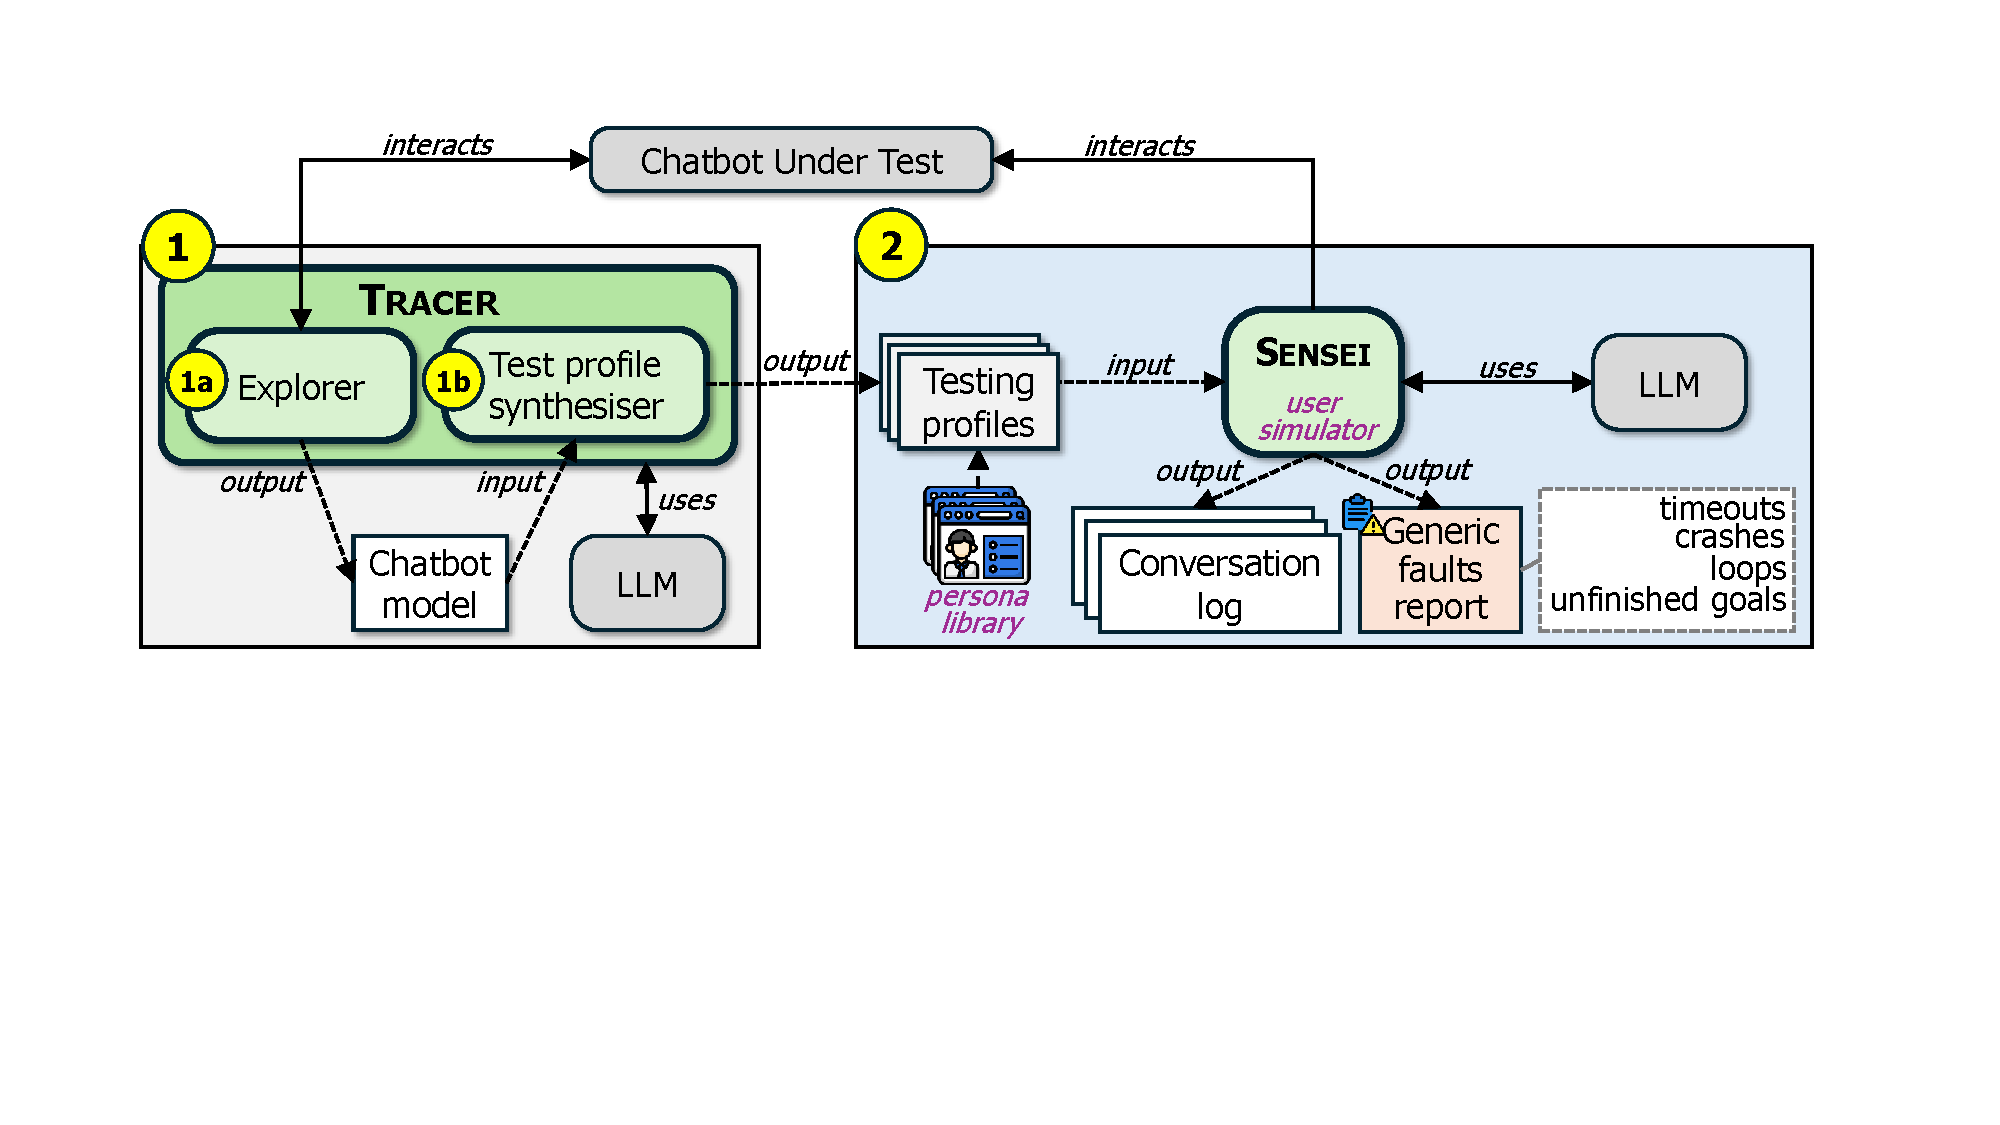
\includegraphics[width=\linewidth]{figures/approach.pdf}
  \caption{Scheme of our approach and its main components.
    (1a) Chatbot’s functionality explorer.
    (1b) Synthesiser of test conversation profiles.
    (2) User simulator.}
  \label{fig:approach}
\end{figure}


\begin{enumerate}
  \item \textbf{Exploration phase (1a):}
    an explorer agent interacts with the chatbot in multiple sessions
    and extracts a model of the chatbot
    The extracted model contains the following information:
    \begin{itemize}
      \item Language(s) that the chatbot understands.
      \item The chatbot's default fallback sentence (e.g., "I'm sorry, I can't undertand what you are saying.")
      \item The functionality graph.
    \end{itemize}

    The functionality graph, as its name implies,
    is a graph, precisely, a \ac{DAG}
    that mimics the workflow of the chatbot.
    Its nodes are functionality nodes,
    an object that contains all the information regarding a functionality
    (will be explained further in 
    \autoref{sec:exploration}).

  \item \textbf{Refinement phase (1b):}
    in this pase the extracted model will be refined,
    similar functionalities will be merged,
    and order of the nodes in the \ac{DAG} will be revised
    so that it matches the chatbot's workflow.
    Once we have this final model,
    the user profiles for SENSEI will be created based on this model.
    The profiles will have goals, context, roles and outputs
    that will match what is found on the model.

  \item \textbf{User simulator (2):}
    Once the model and user profiles have been created,
    we use the profiles within SENSEI, the user simulator.
    During the simulation,
    we can find crashes, conversation loops, timeouts,
    or unfinished goals (i.e., tasks that the user profile had
    but was not able to achieve, like ordering a pizza).
    It is important to note that
    although SENSEI is an important part in this testing process
    it has not been developed in this work.
\end{enumerate}



\section{Exploration Phase}\label{sec:exploration}

The exploration phase is the core of \ac{TRACER}'s modeling.
In this phase, an \ac{LLM} agent interacts with the chatbot under testing
to find its functionalities, language, and fallback
and build a preliminary model.
This is done purely from a black-box perspective
and does not rely on the source code at all.

The explorer agent, inspired by SENSEI
\autocite{delaraSensei, delaraAutomatedEndtoEndTesting2025},
mimics a human interacting with the chatbot
thanks to the use of \acp{LLM}.

\subsection{Initial Probing}

Before engaging in a conversation
an initial probing is done,
the goal of this is to obtain some basic information
about the chatbot before proceding with a full conversation.
It focuses on two elements:

\begin{itemize}
  \item \textbf{Language Detection:}
    The agent determines the language by sending
    some basic messages to the chatbot
    and analyzing the response.
  \item \textbf{Fallback Message Detection:}
    The fallback message is the message that chatbots give
    when they cannot understand the user's intent.
    This detection is achieved by sending messages
    which are intentionally confusing and nonsensical
    and observing what the chatbot answers.
    Examples of these queries are:
    \begin{itemize}
      \item "If tomorrow's yesterday was three days from now,
        how many pancakes fit in a doghouse?"
      \item "Xyzzplkj asdfghjkl qwertyuiop?"
      \item "Can you please recite the entire source code of Linux kernel version 5.10?"
    \end{itemize}
\end{itemize}

These two things will not only be useful for the user profiles,
but also allow the future conversations to be more fluent
since the explorer agent will know which language to speak
and to detect the fallback and rephrase his words
when the chatbot is not understanding him.

\subsection{Iterative Sessions}

After the initial probing,
the explorer agent will have $s$ conversations of $n$ turns each,
where both $s$ and $n$ are configurable parameters.
During this conversations functionalities will be discovered
(see \autoref{subsec:functionality_extraction})
and added to a queue,
this queue will determine what is the goal of the explorer
during each conversation.

\begin{itemize}
  \item \textbf{General Exploration:}
    when the aforementioned queue is empty,
    the explorer will do a general search for functionalities.
    In this type of conversations,
    he will engage in a natural conversation by first greeting the chatbots,
    and then if the chatbots doesn't give away what he can do,
    the explorer will directly ask.
  \item \textbf{Functionality Branch Exploration:}
    in the case that there are functionalities in the queue,
    they will get popped and fed to the explorer agent.
    Then the explorer will have a conversation
    where he will try to find branches and variations of this functionality.
    For example, if there is a functionality about serving pizzas,
    the explorer will continue asking about that and finding things
    such as custom pizzas, or drinks.
\end{itemize}

The purpose of this queue is to explore it in a \ac{DFS} way,
so if we find a functionality, we try to look for branches of it.
This approach was chosen instead of \ac{BFS}
since with \ac{BFS} we cannot know when we have found
all the functionalities of a given depth,
while with this \ac{DFS} approach we could explore a functionality
until we didn't find any variation or branch of it.

\subsection{Functionality Extraction}\label{subsec:functionality_extraction}

At the enf of each conversation,
the Explorer Agent looks at the conversation history
and tries to look for functionalities exhibited by the chatbot.
These functionalities are represented as Functionality Nodes.
As depicted in \autoref{fig:functionality_node},
a Functionality Node contains the following fields:

\begin{figure}[htpb]
  \centering
  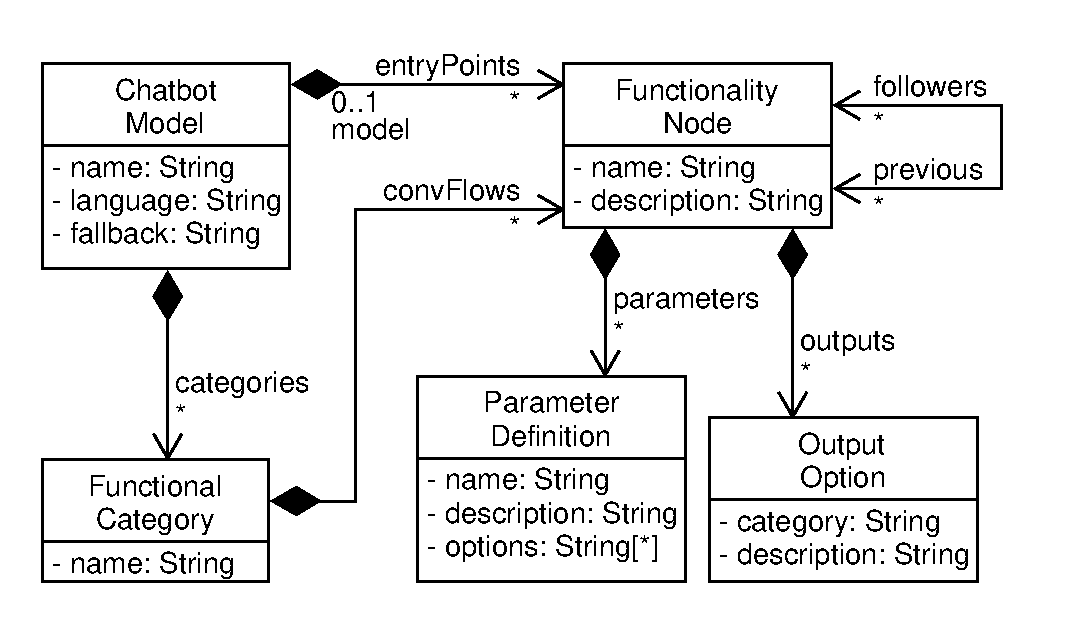
\includegraphics[width=\linewidth]{figures/TRACER_chatbot_model.pdf}
  \caption{
    Chatbot model schema.
  }
  \label{fig:functionality_node}
\end{figure}

\begin{itemize}
  \item \textbf{Name:} the name of the functionality (e.g., \texttt{prompt\_for\_pizza\_size})
  \item \textbf{Description:} what the functionality does (e.g., asks the user for the size of the pizza)
  \item \textbf{Parameters:} fields that the user should input.
    A parameter always has a name and a description
    and optionally can have options.
    This parameter is optional,
    since there are functionalities that don't necessarily need inputs.
    An example of a parameter for the pizza could be this:
    \begin{itemize}
      \item \textbf{Name:} pizza size.
      \item \textbf{Description:} size of the pizza the user wants.
      \item \textbf{Options:} small, medium, large.
    \end{itemize}
  \item \textbf{Output:} as the parameters, outputs are optional.
    It represents pieces of data that we expect the chatbot to output.
    For example when ordering the pizza it could be the price or the order id.
  \item \textbf{Followers and Previous:}
    Since the nodes are aranged as a \ac{DAG},
    the nodes have children and parent
    that mimic the workflow of the chatbot.
    The idea of this workflow graph,
    is to order functionalities in the order that one will encounter them,
    for example, the chatbot will asks for the drinks always after asking for the pizzas
    so then the drink functionality should be a children of the pizza one.
\end{itemize}

On top of this,
the functionalities are clustered into categories.
This is mainly to ease the visual representation for the user
when there are many functionality nodes.

\subsection{Functionality Consolidation}


As the functionality extraction usually results
in the creation of multiple functionality nodes,
the agent performs a consolidation stage where
similar functionalities are merged into a more complete one.
This is achieved in two actions:

\begin{enumerate}
  \item \textbf{Session-Local Merge:}
    first, the functionality nodes extracted during this session
    are compared to one another and with the help of the \ac{LLM}
    semantically similar nodes are merged into a newer, more complete one.
    With this we achieve that the extracted nodes of this session are more relevant.

  \item \textbf{Global Merge:}
    after the nodes discovered in this session have been merged,
    the resulting set is compared with the ones discovered in previous sessions
    and again, the \ac{LLM} look for semantically similar functionalities
    and merges them into one.
\end{enumerate}

To better understand this, we will give an example.
Imagine that throughout the last conversation
we extract a functionality that is called
"prompt for custom pizza ingredients",
with a description that is
"Asks the user to provide the ingredients that he wants on the custom pizza"
but has no parameters or outputs.
Then, in the current session,
the explorer agent's goal is
to find variations or branches of this functionality since is the first in the queue,
and the agent extracts a new functionality called
"prompt ingredients for custom pizza"
with a similar description,
but this time with a list of parameters like
"pepperoni, ham, tuna, olives",
then, the global merge step would merge these two
into a unified version with the parameters.
This was a simple example,
but more complex ones occur where
not only the parameters are added,
but having different lists of parameters they are combined into a more extensive ones,
or the descriptions are combined
to more accurately define what the functionality does.



\section{Refinement Phase}\label{sec:refinement}


Once all the conversation sessions are over,
and the functionalities have been extracted,
we enter the the refinement phase.
The goal of this phase is to take the raw, potentially messy,
functionalities discovered during the exploration phase
and creating a coherent model.

\subsection{Global Consolidation}

While during the exploration phase we have a consolidation phase,
variations of the same functionalities may still appear.
This consolidation step solves this by checking again all the functionality nodes.

\subsection{Chatbot Classification}

Next, based on the discovered functionalities
and the conversation history
the chatbot is classified into informational or transactional.

\begin{itemize}
  \item \textbf{Informational:}
    these are chatbots that mainly answer questions and provide information.
    Examples of these are unversity or bank chatbots that only give you information
    or if you need to do any paperwork they will give you a link and redirect you
    but they will not assist you with the tramit directly.

  \item \textbf{Transactional:}
    these are chatbots that do guide the user
    through a task or workflow.
    For example, the pizzeria example we have been using
    or a hotel chatbot that helps you book a room.
\end{itemize}

\subsection{Workflow Structure Inference}

The final step is to define the \acl{DAG}
that models the chatbot's workflow.
During the exploration phase,
parent-child relationships are set
when a functionality is discovered as a branch or variation from another one,
but most of the nodes are still set as root nodes.
So, we manage to structure this by asking the \ac{LLM}
identify likely sequences, branches, and joins
based on conversational evidence and the dependencies between functionalities.
The prompt for the LLM depends on the chatbot classification:

\begin{itemize}
  \item \textbf{Informational chatbots:}
    usually informational chatbots' functionalities
    don't have parent-child relationships,
    this is because they simply serve information that is not nested through steps.
    This is why this prompt is conservative on the identifications of relations,
    since usually all the questions are entry points
    that can be asked directly.
    So, relationships are only established
    if there is strong evidence that
    a sequence of actions is needed to access the functionality.

  \item \textbf{Transactional chatbots:}
    these other chatbots are more likely to have sequential workflows
    where one functionality will only exhibit
    if a previous action has been done.
    Also, the prompt will look for branches of optional choices,
    for example, ordering a custom pizza or a predefined pizza.
\end{itemize}

\subsection{Example: Inferred Model of a Pizzeria Chatbot}

\autoref{fig:pizzeria-workflow}
shows the workflow graph resulting from a \ac{TRACER} execution
against a pizzeria chatbot built with Taskyto taken from
\autocite{sanchezcuadradoAutomatingDevelopmentTaskoriented2024}.
The entrypoint, represented as a black dot,
is the starting point of a new conversation.
From there, you can go to four different root functionalities
grouped into two categories.
From one of the functionalities,
you can continue the workflow to make your order.
We will now break down the categories and functionalities.

\begin{figure}[htpb]
  \centering
  \includegraphics[width=\linewidth]{figures/workflow_graph-crop-back.pdf}
  \caption{
    Workflow model inferred by \ac{TRACER} from a pizzeria chatbot.
  }
  \label{fig:pizzeria-workflow}
\end{figure}

\begin{itemize}
  \item \textbf{Chatbot Meta:}
    the category contains functionalities related to the chatbot talking about itself.
    It has two functionality nodes, provide welcome message, that as its name says,
    the chatbot will greet the user;
    and state available information,
    in which the chatbot will give information such as
    the opening hours or its capabilities.

  \item \textbf{Order Placement:}
    contains two root functionalities,
    list available pizza types,
    which gives you the flavours of the different pizzas;
    and prompt for pizza details,
    which expects the pizza size and type,
    once this has been completed
    it will continue to ask the user for a confirmation
    and then prompt the user for the type and number of drinks he wishes.

  \item \textbf{Order Confirmation:}
    once the user has gone through all the order placement steps,
    we have the last functionality of the workflow which is
    provide order total,
    here the chatbot will the price of the total order
    and finalize the workflow.
\end{itemize}

This final model can be used for different purposes,
such as reverse engineering, reengineering,
migrating to a different framework
or maintaining the chatbot.
In the next section we will show
how \ac{TRACER} uses this model
to generate user profiles for SENSEI.


% !TeX root = ../main.tex
% Add the above to each chapter to make compiling the PDF easier in some editors.

\chapter{User Profile Structure and Generation}\label{chapter:user_profiles}

Once the model has been finished,
we use it to automatically generate user profiles for SENSEI.
These serve as test cases designed to verify
the discovered functionalities of the chatbot,
its handling of different inputs,
to check if the outputs match the expected value,
and to find other errors such as timeouts.

First, \autoref{sec:profile-structure}
will cover the structure of these profiles and how they work,
then \autoref{sec:profile-generation}
will detail how these profiles are synthesized from the inferred model.


\section{User Profiles Structure}\label{sec:profile-structure}

A user profile contains all the information
that characterises the user,
the conversation goals,
interaction style,
and other information such as the \ac{LLM} that will be used,
or the number of conversations and turn per conversations.
These profiles are structured in a YAML file,
\autoref{code:yaml_profile} shows an example of a user profile generated by \ac{TRACER}.

\begin{figure}[htpb]
  \centering
  \lstinputlisting[
    language=yaml,
    caption={Example of a conversation profile for a pizzeria chatbot.},
    label={code:yaml_profile}
  ]{code/pizza_order_placement.yaml}
\end{figure}

To better understand how the profiles are generated,
we must first understand the profiles and their structure
made up of the \texttt{test\_name},
a unique identifier for the profile,
followed by four configuration blocks: 
\texttt{llm}, \texttt{user}, \texttt{chatbot} and \texttt{conversation}.

\subsection{LLM Configuration (\texttt{llm})}

In this section we can choose the \acl{LLM} that we are going to use
along with its temperature.
The chosen \texttt{model} will have an impact on the achieved results
since each model has its own strengths and limitations
and there will be models that will perform better than others,
usually at the cost of being more expensive.
In this field we will just input the name of the model (e.g. \texttt{gpt-4o-mini}).
Then we have the \texttt{temperature},
this parameter controls the randomness of the \ac{LLM},
that is, when the model is going to choose the next word
how randomly it does it.
A value of 0 means that the model is deterministic
while 1 means that it will be more creative.

\subsection{User Persona Definition (\texttt{user})}

In the \texttt{user} section, we will define
the persona, its role, context and goals.
We start with the \texttt{language} that the user will employ,
followed by the \texttt{role} of the simulated user,
that is, a sentence representing who the user is
and what he ought to do (e.g., A customer ordering a pizza).
The \texttt{context} field provides additional information to the chatbot,
it can add more details or personality traits, such as,
"You are in a hurry", to make the simulated user more realistic.
The \texttt{goals} field is arguably the most important of the user's fields.
In it, we will describe all the objectives for the conversation.
These objectives are written like templates with placeholders
(e.g., Specify the pizza size as {{pizza\_size}}).
Below the list with all the objectives
we have the list of parameters, which is the placeholders we left in goals.
Each of these parameters will have assigned a function:
\begin{itemize}
  \item \texttt{random()}: A random value of the data below will be taken.
  \item \texttt{random(x)}: Takes $x$ different random values.
  \item \texttt{forward()}: Selects one value sequentially from the data list.
  \item \texttt{forward(x)}: Instead of one by one, takes the $x$ next values.
  \item \texttt{forward(var)}: 
    Allows to cycle through all the combinations of a pair (or more, depending on the nested combinations) of variables.
    For example, one could nest pizza sizes with pizza types,
    that means that all combinations of pizza sizes with pizza types would be tested,
    that is, small pepperoni, small four chesee, ..., medium pepperoni, medium four chesee, ..., large pepperoni, large four chesee...
\end{itemize}
After the function, we can specify its \texttt{type},
with values like int, float, string or date.
Right after that, we have the data field,
where we will input a list of values
or if it is a numeric value, a range with min and max
and the step to go from the min to the max.

\subsection{Chatbot Settings (\texttt{chatbot})}

Here, expected behaviour of the system under test will be specified.
The first field is the \texttt{fallback},
this is the sentence given by the chatbot when he cannot understand what the user is saying,
or what he is saying is outside of the chatbot's scope.
Next we have the \texttt{outputs}, a field similar to the goals
but in this case instead of being related to the inputs,
it will be used to extract outputs from the chatbot.
For each output we will give a name
then a \texttt{type} which can be string, money, int, float or date;
then we have a short \texttt{description}.
This information will be used by an \ac{LLM}
to extract the information from the conversation with the chatbot.


\subsection{Conversation Control (\texttt{conversation})}

This last section controls aspects of the execution.
The \texttt{number} will control the number of times the conversation will take place,
the more conversations, the more combinations of the goals' items to be tested.
This field allows an integer, that simply indicates the number of conversations;
\texttt{all\_combinations} that will exhaustively test every combination,
although it ensures good coverage of the inputs,
it can also result in an enormous number of test cases, specially if we use nested forwards;
\texttt{sample(x)}, where $x$ is a number between $0$ and $1$,
will compute all the possible combinations
and take a percentage of all of these.

The second field, \texttt{goal\_style}, is the test's stop condition.
It can be the number of steps taken in the conversation
(let a step be a user message followed by a chatbot's one),
or \texttt{all\_answered} which will stop once the user has completed all of its goals,
this parameter is also accompanied by a \texttt{limit} field which sets a hard limit
making sure that the conversation finishes even if the chatbot is not able to fulfil the user's goals.

Lastly, we have the \texttt{interaction\_style},
which lets us set a list of styles that the simulated user will adopt for its conversations.
This styles are predefined and include some like \textit{make spelling mistakes}, \textit{use short phrases}
or \textit{single question}.

\section{User Profiles Generation}\label{sec:profile-generation}

The profile generation is an automated process
that aims to convert the inferred model
into a set of profiles that will thoroughly test the chatbot.
The process is divided into seven steps that begins by
grouping functionalities into profiles,
followed by the \ac{LLM}-driven generation of goals, variables, context, and outputs.
Then, the definition of the conversation style and,
finally, the profile assembly and validation step.
Each of these steps is detailed in the following subsections.

\subsection{Grouping Functionalities into Profiles}

The inferred model is send to an \ac{LLM} along with conversation fragments,
with this information the \ac{LLM} is prompted to
group the functionalities into realistic and logical user scenarios.
Each group will gather functionalities that are semantically related,
frequently used together or performed sequentially.
Ideally, each functionality is only assigned to one group
to ensure that all functionalities are used but avoiding redundancy;
this is not always achieved since in cases where a functionality branches into others
it is required to go through it at least twice.
From this functionality groups, the \ac{LLM} will generate
the \texttt{test\_name} along with its \texttt{role}.

\subsection{Goal Generation}

After the grouping has been done,
the group of functionalities is sent to a new \ac{LLM} call
that will create a set of functionalities that when fulfilled
will ensure that the functionalities have been activated.
The goals may or may not have variables,
it will depend on the nature of the goal,
for example if asking about the opening hours it will not have variables,
but if the goal is about asking for a pizza,
then the goal will likely have variables.

\subsection{Variable Generation}

This step is only needed when variable \texttt{\{\{placeholders\}\}} have been defined.
To understand how the variables are generated first we need to see waht a data source is.
A data source are the values of either a parameter or an output from a functionality node,
we decided to use both outputs and parameters since there are occasions
where the extracted functionality is for example "list available pizza types"
and the values that we can use for the variables
are in the outputs instead of the more obvious parameters.
So the data sources are the combinations of all the values
from all outputs and parameters.

Now that we now this, the procedure is as follows for each individual variable.
First, we pass all these data sources to the \ac{LLM}
and prompt it to match the variable to one of the data sources
emphasizing that it is not necessary to force a match
just for the sake of making one.
Then, if one match is given,
we request the \ac{LLM} to generate another extra value
based on what the returned data source
to test the chatbot on values outside of the ones that he suggests.
For example, with the pizza sizes small, medium, large,
it tends to generate extra large as the extra value.

In the case that no data source is matched,
either because the chatbot didn't provide values
(for example with dates or numbers)
or because the data source matching didn't correctly match the variable,
the \ac{LLM} will generate the data for the variable given
the goals, functionalities, role and conversations.

The generated variables always use the \texttt{forward()} function
since it allows us to test every option.
We chose this over the nested one
since it has a great balance between completeness and number of conversations.
For example, having $8$ pizza types with $3$ different pizza sizes
with nested forwards would require $8 \cdot 3 = 24$ conversations,
while using the regular forward would require only $8$ conversations
to go through all the options.

\subsection{Context Generation}

A simple context of two or three sentences
is generated by the \ac{LLM} based on
the functionalities, the content generated before and the conversations.
The idea of the generated context is to create a more realistic scenario
where the user is not simply testing the chatbot
but in a realistic case where for example
the user is in a get together is looking to order pizzas,
or is an Erasmus student requesting help to a university chatbot.

\subsection{Output Definition}

The output definition along with the goal and variables is one of the key steps.
It will let us test the chatbot
and see if the chatbot is returning the information that it should
and thus completing its functionalities.
The outputs are generated by the \ac{LLM}
taking into account the functionality and the goals,
trying to look for things that will ensure that they have been achieved,
like for example the order ID or the order price;
and by also looking at the outputs from the functionality nodes.

These outputs are as granular as possible
to allow for a better testing of the chatbot,
for example, instead of a more vague output like
"order confirmation", it would be split into two granular outputs
"order ID" and "total order price".

\subsection{Conversation Style Definition}

The \texttt{conversation} section does not require \ac{LLM} calls.
First, the number of conversations is chosen
based on the variable with the largest data set,
for instance, if we have four variables,
and pizza type, with $8$ options, is the one with the larger set of options,
the number of conversations will be $8$ to ensure that all the variables are tested.

For the length of the conversation,
we went for a limit that is set based
on a linear combination of the number of goals and outputs,
so that the greater the number of goals and outputs,
the longer the conversation will be,
but still with a hard limit of $30$.

\subsection{Profile Assembly and Validation}

Once all the fields have been generated
the profile is turned into a YAML profile.
This profile is then passed through a validation script
that will check things like that all the required fields are complete,
that every placeholder has a variable defined,
and that this one is correctly defined
amongst other things,
and if any error appears it will return a verbose description of the issue.
Then, if any error arises, the description along with the YAML file
are sent to the \ac{LLM} with a prompt to fix the issue.


This seven steps allow us to turn the inferred model
from the deployed chatbot under test,
into a set of realistic and comprehensive user profiles
that will act as test cases when combined with the user simulator Sensei.
This profile generation stage bridges the gap between
black-box model inference and automated testing.

% !TeX root = ../main.tex
% Add the above to each chapter to make compiling the PDF easier in some editors.

\chapter{Tool Support}\label{chapter:tool_support}

To ensure that the previous methodology can be reproduced
we have implemented \acf{TRACER} in an open-source Python package
to allow users to execute it from a \ac{CLI}.
On top of that, we have developed a web application
that allows users to execute both \ac{TRACER} and Sensei
without the need of knowing how to operate the command line.


\section{Implementation and Architecture}

\subsection{Core Framework: LangGraph}

As explained during the \autoref{sec:profile-generation} (\nameref{sec:profile-generation})
\ac{TRACER} relies on \acp{LLM},
this is why used LangGraph \autocite{LangGraph} as our framework for development.
The reason why we chose LangGraph
was because it allows to manage and orchestrate
complex agentic workflows with states,
it is also an industry standard and
it has an extensive documentation.
LangGraph allows us to orchestrate the different stages
and to keep complex states where we store
the inferred model and the fields generated for the profiles.
Right now \ac{TRACER} allows OpenAI and Gemini models,
but thanks to LangGraph it would be easy to add other \ac{LLM} providers.

\subsection{Modular Architecture}

\ac{TRACER} can infer a chatbot model as long as
the chabots is accessible through an interface, typically a \acs{REST} \acs{API}.
Right now it provides access to communicate with chatbots made with different technologies,
such as Taskyto \autocite{sanchezcuadradoAutomatingDevelopmentTaskoriented2024}, Rasa \autocite{Rasa2020} or 1MillionBot \autocite{1MillionBot}.
In addition, new connectors could be added by extending the current implementation.

Apart from these connectors,
\ac{TRACER} is divided into three modules,
each corresponding to a phase of the methodology:

\begin{itemize}
  \item \textbf{Explorer Module:}
    Contains the Explorer Agent
    and implements the logic for the Exploration Phase (see \autoref{sec:exploration}),
    managing the conversational sessions and the initial extraction of Functionality Nodes.

  \item \textbf{Refinement Module:}
    Implements the logic for the Refinement Phase (see \autoref{sec:refinement}),
    responsible for consolidating functionalities,
    classifying the chatbot, and inferring the final workflow structure.

  \item \textbf{Profile Generation Module:}
    Implements the seven-step synthesis process (see \autoref{sec:profile-generation}),
    taking the final chatbot model and generating the YAML user profiles.
\end{itemize}

\subsection{Generated Artifacts}

Upon completion, \ac{TRACER} generates the following artifacts
containing the results from the full analysis performed on the target chatbot:

\begin{itemize}
  \item A set of user profiles
    representing realistic users that would use the application
    and that will act as test cases
    (see \autoref{code:yaml-profile-pizza} and \autoref{code:yaml-profile-drinks})
  \item A markdown report containing the inferred model information like
    the discovered functionalities, fallback message, language
    and also other information like token usage, number of \ac{LLM} calls or estimated cost.
  \item A graph representing the inferred model's workflow (see \autoref{fig:pizzeria-workflow})
  \item A JSON file containing the same workflow but in text.
\end{itemize}



\section{Distribution and Development Workflow}

Before detailing the \ac{CLI}'s functioning,
this section will describe \ac{TRACER}'s packaging, distribution,
and the software engineering practices used to maintain its quality.
\ac{TRACER} is packaged and distributed as a package on the \acf{PyPI} repository
(\url{https://pypi.org/project/chatbot-tracer/}),
making it easy to install by running
\texttt{pip install chatbot-tracer}.
This not only makes it easy to use,
but also makes it easy to implement into other projects
such as the web application done,
or other projects that could use \ac{TRACER}
since it can just be added as another package requirement.

To ensure code quality and automate the release process
\ac{TRACER} makes use of GitHub Actions for the \ac{CI/CD} pipeline.
For the \ac{CI} we made use of Ruff \autocite{Ruff}.
Ruff is Python linter and formatter written in Rust
that combines tools like Flake8 or Black into a single and faster tool.
We made use of Ruff not only to enforce a consistent code style,
but also to enforce code quality standards,
such as ensuring proper documentation
and managing code complexity by setting thresholds for metrics like McCabe's cyclomatic complexity.
For the \ac{CD} side,
we implemented a pipeline that whenever a tag with the format \texttt{v*.*.*} is published
automatically builds the package,
publishes it to \ac{PyPI},
and creates the corresponding GitHub release.
All the \ac{TRACER} source code can be accessed in \url{https://github.com/Chatbot-TRACER/TRACER}.

\section{The \acl{CLI}}

The primary way of using \ac{TRACER} is through the \ac{CLI}.
We can execute the whole \ac{TRACER} pipeline,
from chatbot exploration to profile generation,
through a single command.
This way enables users who prefer terminal-based workflows
such as developers, to execute TRACER easily.
It also allows \ac{TRACER} to be integrated within other projects.

\ac{TRACER} is run by one main command: \texttt{tracer}.
To see in more detail its options, users can run \texttt{tracer --help}.
Some of the key arguments are the following ones:

\subsection{Conversation Control}

\texttt{--sessions} or \texttt{-s} that controls the number of conversations
that \ac{TRACER} will have with the chatbot under testing
and \texttt{--turns} or \texttt{-n} for the number of turns or steps per conversation.

\subsection{Connector Configuration}

The arguments \texttt{--technology} or \texttt{-t} along with \texttt{--url} or \texttt{-u}
allow to configure the connector by choosing
the chatbot technology along with the \ac{API} endpoint.

\subsection{LLM Configuration}

Using \texttt{--model} or \texttt{-m} lets one decide the \acl{LLM} used for the exploration and analysis,
then \texttt{--profile-model} or \texttt{-pm} is an optional argument
that if set will make the generated user profiles' \ac{LLM} be the one specified,
otherwise the \ac{LLM} that will appaer in the profiles will be the same one used for \ac{TRACER},
it is recommended to use a better model for exploration and analysis
since will infer a more comprehensive model with more realistic profiles,
and then a more economic model to run the profiles
since there will be many more \ac{LLM} calls
and the chosen model will not have that much impact.

\subsection{Output and Logging}

We also have the verbose levels which can be three levels:
the basic one where we will just see things like the discovered functionalities,
which session or phase are we in and warnings.
The verbose level, activated with \texttt{-v},
which allows us to see the conversation too,
and the debug \texttt{-vv} that will show what the verbose shows plus information like
prompts sent to the \ac{LLM}, its responses,
and other logs that may have been set during the development and debugging of the program.
Lastly, we have \texttt{--output} or \texttt{-o},
which simply controls where all the generated artifacts will be placed.

\begin{lstlisting}[
language=bash,
caption={Tracer command example.},
label={code:tracer-command-example}
]
$ tracer -t taskyto -u http://localhost:5000 -s 12 -n 8 -m gemini-2.5-flash -pm gemini-2.0-flash -o ./pizzeria_results -v
\end{lstlisting}

The command in \autoref{code:tracer-command-example}
demonstrates a typical execution of \ac{TRACER} against a Taskyto-based pizzeria chatbot. 
It is configured to run 12 exploration sessions of 8 turns each.
For the exploration, analysis and profile generation, the smarter model Gemini 2.5 Flash will be used,
then for the model that is defined in each user profile, Gemini 2.0 Flash will be used since it is faster and cheaper.
We used the \texttt{-v} to be able to monitor the conversations that are happening
between the explorer agent and the chatbot under testing.
Finally, all the artifacts will be stored in a directory called \texttt{pizzeria\_results}.

\section{The Web Application}

To complement the \ac{CLI},
we developed a web application
to provide a user friendly interface that will allow to run the whole end-to-end pipeline,
that it is, to run \ac{TRACER} to generate the user profiles,
and then to execute these with Sensei.
This, allows a broader audience to use both \ac{TRACER} and Sensei
without the need of knowing how to use the \ac{CLI}.

\subsection{System Architecture}

\subsection{Core Technology Stack}

The backend of the application was developed in Django \autocite{Django},
the reason why this framework was used is because it is made for Python
so it suits both \ac{TRACER} and Sensei,
and also it offers the Django REST Framework \autocite{DjangoRESTFramework}
that will allow us to develop a \ac{REST} \ac{API} that will be consumed by our frontend.

For the frontend we went with React \autocite{React},
a JavaScript library to develop \acp{SPA}
that will consume directly from our Django \ac{API}.

Lastly, to ensure data persistance,
we used PostgreSQL \autocite{PostgreSQL2025},
we chose a \ac{SQL} database since Django's \ac{ORM} supports this type of databases out of the box,
also, we preferred PostgreSQL over the default Django's SQLite
since the latter is more oriented to development and testing
and stores everything in a single file which causes concurrency and performance issues when used in production.

\subsection{Asynchronous Task Handling}

\ac{TRACER} and Sensei executions both take from a few minutes up to hours,
thus, executing this tasks synchronously would leave the user's interface frozen
for the duration of the whole process.
To handle this we implemented asynchronous executions,
we did this by using a distributed task queue called Celery \autocite{Celery},
which lets us handle these jobs asynchronously.
Then, to communicate Django with Celery we need a broker,
for this we used RabbitMQ \autocite{RabbitMQ}.
These two tools in conjunction will allow the user to execute \ac{TRACER} or Sensei
and change to a different view, log out, or even turn off the computer
and then come back to check the progress.
It will also help the server to not get saturated
since we can limit the number of concurrent jobs
and if there are requests to execute more than this number,
the jobs will be waiting on the queue instead of saturating the server.


\subsection{The Nginx Reverse Proxy}

\begin{figure}[ht]
    \centering
    \begin{tikzpicture}[
        node distance=1.5cm,
        box/.style={rectangle, draw, fill=blue!20, text centered, minimum height=1cm, minimum width=2.5cm, align=center},
        client/.style={rectangle, draw, fill=green!20, text centered, minimum height=1cm, minimum width=2.2cm, align=center},
        storage/.style={rectangle, draw, fill=orange!20, text centered, minimum height=1cm, minimum width=2.2cm, align=center},
        backend/.style={rectangle, draw, fill=yellow!20, text centered, minimum height=1cm, minimum width=2.2cm, align=center},
        arrow/.style={->, thick, align=center},
        scale=0.9
    ]

    % Client
    \node[client] (client) {Client Browser\\Port 80};

    % Nginx
    \node[box, below=of client] (nginx) {Nginx Proxy\\Port 8080};

    % Destinations arranged vertically for better fit
    \node[storage, below left=1.2cm and 1.2cm of nginx] (react) {React Files\\/var/www/react};
    \node[storage, below=1.2cm of nginx] (static) {Static Files\\/var/www/static};
    \node[backend, below right=1.2cm and 1.2cm of nginx] (backend) {Django API\\backend:8000};

    % Arrows from client to nginx
    \draw[arrow] (client) -- (nginx);

    % Arrows from nginx to destinations
    \draw[arrow] (nginx) -- node[above left, font=\footnotesize] {/} (react);
    \draw[arrow] (nginx) -- node[right, font=\footnotesize] {/static/} (static);
    \draw[arrow] (nginx) -- node[above right, font=\footnotesize] {/api/, /admin/,\\/filevault/} (backend);

    \end{tikzpicture}
    \caption{Nginx routing to serve React, Django's static files and Django API.}
    \label{fig:nginx-routing}
\end{figure}


\subsection{Deployment and Containarization}

\begin{figure}[ht]
    \centering
    \resizebox{\linewidth}{!}{
    \begin{tikzpicture}[
        node distance=2.2cm,
        container/.style={rectangle, draw, thick, text centered, minimum height=0.5cm, minimum width=3cm, align=center},
        volume/.style={cylinder, draw, fill=gray!20, text centered, minimum height=0.15cm, minimum width=1.8cm, aspect=0.3, align=center},
        dependency/.style={->, dashed, thick, red},
        mount/.style={-, thick, blue},
        scale=1.0
    ]


    % Shared Volumes at top
    \node[volume] (filevault) at (6, 6.5) {filevault\_data\_prod};
    \node[volume] (reactbuild) at (-5, 6.5) {react\_build};

    % Top: NGINX
    \node[container, fill=orange!20] (nginx) at (0.5, 9.2) {nginx:latest\\Port 80→8080};

    % Mid: Frontend | Backend | Celery
    \node[container, fill=green!20] (frontend) at (-5, 4.2) {Frontend\\React Build};
    \node[container, fill=yellow!20] (backend) at (-0.2, 4.2) {Backend\\Django API\\Port 8000};
    \node[container, fill=blue!20] (celery) at (5, 4.2) {Celery Worker\\Async Tasks};

    \node[volume] (staticfiles) at (2, 6.7) {static\_files\_prod};

    % Lower: DB | RabbitMQ
    \node[container, fill=cyan!20] (db) at (-2, 1.3) {postgres:16\\Port 5432};
    \node[container, fill=pink!20] (rabbitmq) at (2.5, 1.3) {rabbitmq:3-mgmt\\Port 5672};

    % Volumes at bottom
    \node[volume] (pgdata) at (-2, -1) {postgres\_data};
    \node[volume] (rmqdata) at (2.5, -1) {rabbitmq\_data};

    % Dependency arrows (red dashed)
    \draw[dependency] (backend) -- (db);
    \draw[dependency] (backend) -- (rabbitmq);
    \draw[dependency] (celery) -- (db);
    \draw[dependency] (celery) -- (rabbitmq);
    \draw[dependency] (frontend) -- (backend);
    \draw[dependency] (nginx) -- (backend);
    \draw[dependency] (nginx) -- (frontend);

    % Volume mounts (blue solid)
    \draw[mount] (db) -- (pgdata);
    \draw[mount] (rabbitmq) -- (rmqdata);
    \draw[mount] (frontend) -- (reactbuild);

    \draw[mount] (filevault) -- (backend);
    \draw[mount] (filevault) -- (celery);
    \draw[mount] (staticfiles) -- (backend);
    \draw[mount] (staticfiles) -- (celery);
    \draw[mount] (staticfiles) -- (nginx);
    \draw[mount] (staticfiles) -- (frontend);
    \draw[mount] (reactbuild) -- (nginx);

    % Legend at bottom
    \node[font=\small] at (-5.5, -2.4) {Legend:};
    \draw[dependency] (-5, -2.7) -- (-4.3, -2.7);
    \node[font=\footnotesize, anchor=west] at (-4.1, -2.7) {Container Dependencies};
    \draw[mount] (-5, -3.0) -- (-4.3, -3.0);
    \node[font=\footnotesize, anchor=west] at (-4.1, -3.0) {Volume Mounts};

    \end{tikzpicture}
    }
    \caption{Docker Container Architecture.}
    \label{fig:docker-architecture}
\end{figure}

% !TeX root = ../main.tex
% Add the above to each chapter to make compiling the PDF easier in some editors.

\chapter{Evaluation}\label{chapter:evaluation}

In this section we aim to
evaluate how \ac{TRACER} perfoms at
modelling and synthesising user profiles
from a chatbot under testing.
To do so we will answer the following research questions:

\begin{itemize}
\item \textbf{RQ1: How effective is TRACER in modeling chatbot functionality?}
  This question evaluates the capability of our model discovery method to attain high functional coverage in a controlled environment where the ground truth is available.
\item \textbf{RQ2: How effective are the synthesised profiles at detecting faults in controlled environments?}
  This question tests the accuracy of our method by applying mutation testing \autocite{gomez-abajoMutationTestingTaskOriented2024} to estimate the capacity of the created profiles to detect specific, injected faults.
\item \textbf{RQ3: How accurately does TRACER model the functionalities of real-world, deployed chatbots?}
  This question addresses the practical, real-world applicability of \ac{TRACER}.
  To answer it, we will compare the inferred model against a handmade one
  of deployed chatbots
  and measure the precission, recall and F1-score.
\end{itemize}

RQ1 evaluates the coverage of our approach
in terms of activating chatbot functionalities.
To measure the coverage, \ac{TRACER} will be executed
against the chatbot under testing
and the generated synthesised profiles
will be executed with SENSEI against the same chatbot.
We will perform this with chatbots created with the Taskyto framework
because this framework offers the possibility
of reporting the activated modules.
With these reports we will be able to measure
the coverage obtained during the \ac{TRACER} and SENSEI executions independently.

We anticipate higher coverage during SENSEI profile execution,
as profiles are designed to systematically test all discovered parameters
and their valid combinations.
For instance, \ac{TRACER} may find that a pizzeria chatbot
offers six pizza types, but does not try them all during exploration;
instead, the generated profiles are designed to test all options.

Evaluating RQ1 is crucial for understanding
how thoroughly \ac{TRACER} exercises the chatbot’s functionality.
High coverage does not guarantee high quality,
but it implies that a significant part of a system has been tested,
increasing the confidence in its reliability
\autocite{ammannIntroductionSoftwareTesting2017}.


RQ2 assesses the practical effectiveness
of our approach in detecting chatbot errors.
To this aim, we employ mutation testing
\autocite{demilloHintsTestData1978}
by introducing defects into correct chatbots to create mutants,
and testing whether the generated profiles detect these defects.
A profile successfully detects a mutation (i.e., a fault)
when the simulated user fails to complete a goal
(e.g., ordering a pizza type that was removed in the mutant)
or when an expected output is missing or incorrect
This way, assessing RQ2 is important
to provide evidence that our approach produces
profiles that are sufficiently comprehensive
to reveal real-world chatbot errors.

RQ3 assesses \ac{TRACER}'s ability at modeling and synthesising
real-world deployed chatbots.
Contrary to RQ1 and RQ2 that work with chatbots developed with \ac{TRACER} framework
specifically for this evaluation,
RQ3 evaluates chatbots deployed for real-world applications
such as, universities, townhalls or transportation companies.
To evaluate this, we will craft a hand-made model
by interacting with the chatbot
and then compare it with the one inferred by \ac{TRACER}.

% !TeX root = ../main.tex
% Add the above to each chapter to make compiling the PDF easier in some editors.

\chapter{Conclusions and Future Work}\label{chapter:conclusion}




\appendix{}

\microtypesetup{protrusion=false}

\addchap{Abbreviations}
\begin{acronym}
	\itemsep-.25\baselineskip
	\acro{TUM}[TUM]{Technical University of Munich}
  \acro{UAM}[UAM]{Universidad Autónoma de Madrid}
  \acro{EPS}[EPS]{Escuela Politécnica Superior}
  \acro{AI}[AI]{Artificial Intelligence}
  \acro{NLP}[NLP]{Natural Language Processing}
  \acro{RAG}[RAG]{Retrieval-Augmented Generation}
  \acro{LLM}[LLM]{Large Language Model}
  \acro{DSL}[DSL]{Domain-Specific Language}
  \acro{TRACER}[TRACER]{Task Recognition And Chatbot ExploreR}
  \acro{BDR}[BDR]{Bug Detection Rate}
  \acro{TCR}[TCR]{Task Completion Rate}
  \acro{CLI}[CLI]{Command Line Interface}
  \acro{API}[API]{Application Programming Interface}
  \acro{JSON}[JSON]{JavaScript Object Notation}
  \acro{PyPI}[PyPI]{Python Package Index}
  \acro{NLU}[NLU]{Natural Language Understanding}
  \acro{DAG}[DAG]{Directed Acyclic Graph}
\end{acronym}

\listoffigures{}
\listoftables{}
\microtypesetup{protrusion=true}
\printbibliography{}

\end{document}
